
\begin{figure*}
\resizebox{\linewidth}{!}{ % Automatically scales diagram to fit page width
\begin{tikzpicture}[
    function/.style={rectangle, draw, rounded corners, minimum width=2cm, minimum height=1cm, text centered, node distance=1cm},
    distribution/.style={ellipse, draw, minimum width=1cm, minimum height=0cm, text centered, node distance=0.1cm},
    gaussian/.style={draw, smooth, samples=100, domain=-2.5:2.5},
    NPSK/.style={rectangle, draw, rounded corners, minimum width=2.5cm, minimum height=1cm, text centered, node distance=1.5cm, fill=blue!20},
    level 1/.style={sibling distance=6cm, level distance=1cm},
    level 2/.style={sibling distance=2cm, level distance=1.2cm},
    mss/.style={fill=red!50, draw=black},
    ploss/.style={fill=blue!50, draw=black},
    likert/.style={fill=green!40, draw=black}
]

% Existing functions and distributions diagram
\node[function] {Synthesizer Program}
    child { node[function] {DTW\_Onset}
        child { node[distribution, mss] {MSS}
            child[grow=down, level distance=1cm] {
                node[draw=none] {
                    \begin{tikzpicture}[scale=0.7]
                        \draw[red] plot (\x/3, {exp(-\x*\x)});  % Red Gaussian
                    \end{tikzpicture}
                }
            }
        }
        child { node[distribution, ploss] {P-Loss}
            child[grow=down, level distance=1cm] {
                node[draw=none] {
                    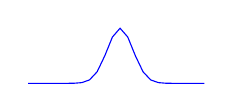
\begin{tikzpicture}[scale=0.7]
                        \draw[blue] plot (\x/3, {exp(-\x*\x)});  % Blue Gaussian
                    \end{tikzpicture}
                }
            }
        }
        child { node[distribution, likert] {Likert}
            child[grow=down, level distance=1cm] {
                node[draw=none] {
                    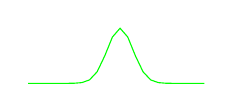
\begin{tikzpicture}[scale=0.7]
                        \draw[green] plot (\x/3, {exp(-\x*\x)});  % Green Gaussian
                    \end{tikzpicture}
                }
            }
        }
    }
    child { node[function] {L1\_Spec}
        child { node[distribution, mss] {MSS} }
        child { node[distribution, ploss] {P-Loss} }
        child { node[distribution, likert] {Likert} }
    }
    child { node[function] {SIMSE\_Spec}
        child { node[distribution, mss] {MSS} }
        child { node[distribution, ploss] {P-Loss} }
        child { node[distribution, likert] {Likert} }
    }
    child { node[function] {JTFS}
        child { node[distribution, mss] {MSS}
            child[grow=down, level distance=1cm] {
                node[draw=none] {
                    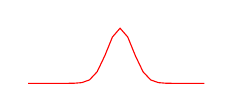
\begin{tikzpicture}[scale=0.7]
                        \draw[red] plot (\x/3, {exp(-\x*\x)});  % Red Gaussian
                    \end{tikzpicture}
                }
            }
        }
        child { node[distribution, ploss] {P-Loss}
            child[grow=down, level distance=1cm] {
                node[draw=none] {
                    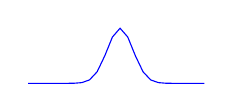
\begin{tikzpicture}[scale=0.7]
                        \draw[blue] plot (\x/3, {exp(-\x*\x)});  % Blue Gaussian
                    \end{tikzpicture}
                }
            }
        }
        child { node[distribution, likert] {Likert}
            child[grow=down, level distance=1cm] {
                node[draw=none] {
                    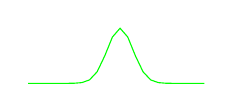
\begin{tikzpicture}[scale=0.7]
                        \draw[green] plot (\x/3, {exp(-\x*\x)});  % Green Gaussian
                    \end{tikzpicture}
                }
            }
        }
    };

% Label for the second row (Distributions)
\node at (0,-3.25) {\textbf{$\longleftarrow$\ \ \large Bootstrapped Distributions\ \ $\longrightarrow$}};
% Left side: NPSK with MSS

\def\xoffsetL{-0.5}
\def\xoffsetM{0}
\def\xoffsetR{0.5}
\def\yoffset{1}

% Left: NPSK with MSS
\node[NPSK, text height=5ex, align=center, fill=red!30, draw=black] at ({-6+\xoffsetL},{-6+\yoffset}) {NPSK with 4 \\ MSS distributions};
\draw[->] ({-6+\xoffsetL},{-6.5+\yoffset}) -- ({-6+\xoffsetL},{-6.6+\yoffset}) node[below, below] {\textbf{Ranks 1-4}};
\draw[red!40, thick] ({-5+\xoffsetL}, {-5.4+\yoffset}) -- ({-2.95+\xoffsetL}, {-5.15+\yoffset});  % Line 1
\draw[red!40, thick] ({-5.5+\xoffsetL}, {-5.4+\yoffset}) -- ({-3.5+\xoffsetL}, {-4.75+\yoffset});  % Line 2
\draw[red!40, thick] ({-6+\xoffsetL}, {-5.4+\yoffset}) -- ({-5.5+\xoffsetL}, {-4.75+\yoffset});  % Line 3
\draw[red!40, thick] ({-6.5+\xoffsetL}, {-5.4+\yoffset}) -- ({-9+\xoffsetL}, {-4.75+\yoffset});  % Line 4

% Middle: NPSK with P-Loss
\node[NPSK, text height=5ex, align=center, fill=blue!40, draw=black] at ({0+\xoffsetM},{-6+\yoffset}) {NPSK with 4 \\ P-Loss distributions};
\draw[->] ({0+\xoffsetM},{-6.5+\yoffset}) -- ({0+\xoffsetM},{-6.6+\yoffset}) node[below, below] {\textbf{Ranks 1-4}};
\draw[blue!40, thick] ({1.5+\xoffsetM}, {-5.4+\yoffset}) -- ({3.25+\xoffsetM}, {-4.75+\yoffset});  % Line 1
\draw[blue!40, thick] ({0.75+\xoffsetM}, {-5.4+\yoffset}) -- ({1.5+\xoffsetM}, {-4.75+\yoffset});  % Line 2
\draw[blue!40, thick] ({-0.25+\xoffsetM}, {-5.4+\yoffset}) -- ({-1+\xoffsetM}, {-4.75+\yoffset});  % Line 3
\draw[blue!40, thick] ({-0.75+\xoffsetM}, {-5.4+\yoffset}) -- ({-3+\xoffsetM}, {-4.75+\yoffset});  % Line 4

% Right: NPSK with Likert
\node[NPSK, text height=5ex, align=center, fill=green!30, draw=black] at ({6+\xoffsetR},{-6+\yoffset}) {NPSK with 4 \\ Likert distributions};
\draw[->] ({6+\xoffsetR},{-6.5+\yoffset}) -- ({6+\xoffsetR},{-6.6+\yoffset}) node[below, below] {\textbf{Ranks 1-4}};
\draw[green!50, thick] ({7.5+\xoffsetR}, {-5.4+\yoffset}) -- ({8.75+\xoffsetR}, {-5+\yoffset});  % Line 1
\draw[green!50, thick] ({6.75+\xoffsetR}, {-5.4+\yoffset}) -- ({6+\xoffsetR}, {-4.75+\yoffset});    % Line 2
\draw[green!50, thick] ({5.75+\xoffsetR}, {-5.4+\yoffset}) -- ({4+\xoffsetR}, {-4.85+\yoffset});    % Line 3
\draw[green!50, thick] ({4.95+\xoffsetR}, {-5.4+\yoffset}) -- ({3.25+\xoffsetR}, {-5.1+\yoffset}); % Line 4



\end{tikzpicture}
}
\caption{For each synthesizer program, we assign ranks to the four loss functions  (\DTWEnv, \LoneSpec, \SIMSESpec, \JTFS) in three different ways, using MSS, P-Loss, or manually assigned Likert scores.}
\label{fig:posthoc_evaluation}
\end{figure*}